\documentclass[11pt,xcolor=x11names,compress]{beamer}

%\usetheme{Berlin}
\usepackage{cmap}					% поиск в PDF
\usepackage{mathtext} 				% русские буквы в формулах
\usepackage[T2A]{fontenc}			% кодировка
\usepackage[utf8]{inputenc}			% кодировка исходного текста
%\usepackage[english,russian]{babel}	% локализация и переносы
\usepackage{array}
\usepackage{amsmath,amsfonts,amssymb,amsthm,mathtools} % AMS

%%% Работа с картинками
\usepackage{graphicx}  % Для вставки рисунков
%\usepackage{booktabs}% Для вставки таблиц
%%% Картинки
\usepackage{tikz} % Работа с графикой
\usetikzlibrary{decorations.fractals}
\usepackage{pgfplots}
\usepackage{pgfplotstable}
\usepackage[textfont={footnotesize}]{caption}

%% Beamer Layout %%%%%%%%%%%%%%%%%%%%%%%%%%%%%%%%%%
\useoutertheme[subsection=false,shadow]{miniframes}
\useinnertheme{default}
\usefonttheme{serif}
\usepackage{palatino}
\usepackage{color}
\usepackage{amsmath}


\setbeamerfont{title like}{shape=\scshape}
\setbeamerfont{frametitle}{shape=\scshape}

\setbeamercolor*{lower separation line head}{bg=Green3} 
\setbeamercolor*{normal text}{fg=black,bg=white} 
\setbeamercolor*{alerted text}{fg=red} 
\setbeamercolor*{example text}{fg=black} 
\setbeamercolor*{structure}{fg=black} 
 
\setbeamercolor*{palette tertiary}{fg=black,bg=black!10} 
\setbeamercolor*{palette quaternary}{fg=black,bg=black!10} 

\setbeamertemplate{footline}[frame number]
\setbeamerfont{page number in head/foot}{size=\normalsize}
\setbeamertemplate{caption}{\raggedright\insertcaption\par}

\DeclareMathOperator*{\argmin}{arg\,min}
\DeclareMathOperator{\E}{\mathbb{E}}

\renewcommand{\(}{\begin{columns}}
\renewcommand{\)}{\end{columns}}
\newcommand{\<}[1]{\begin{column}{#1}}
\renewcommand{\>}{\end{column}}
%%%%%%%%%%%%%%%%%%%%%%%%%%%%%%%%%%%%%%%%%%%%%%%%%%




\captionsetup{justification=centering}
\setbeamertemplate{bibliography item}[text]
\bibliographystyle{apalike}

%\captionsetup{font=scriptsize,labelfont=scriptsize}

\title{\textbf{Opening the black box of Deep Neural Networks
via Information}}
\date{
	\begin{tikzpicture}[decoration=Koch curve type 1] 
		\draw[Green4] decorate{ decorate{ decorate{ (0,0) -- (3,0) }}}; 
	\end{tikzpicture}  
	\\
	\vspace{1cm}
	April 29, 2017
}
\author{Ravid Schwarz-Ziv \and Naftali Tishby}
\institute{Presentation by Bogdan Kirillov for Graphical Models and Statistical Inference mini-course at Skoltech}
\usepackage{graphicx}
\begin{document}

\begin{frame}[noframenumbering]
	\titlepage
\end{frame}

\begin{frame}
	\frametitle{Key points of the paper}
	\begin{itemize}
		\item Most of the training time is spent on compression of the input to efficient representation rather than on fitting to labels;
		\item The compression begins when the training errors shrink and the SGD epochs go into random diffusion, constrained by the training error value;
		\item The converged layers lie very close to the theoretical bound, and the maps from the input to any hidden layer and from this hidden layer to the output satisfy the IB self-consistent equations. This mechanism is absent in one layer networks;
		\item Adding more hidden layers reduces training time;
		\item Hidden layers are expected to converge to critical points for phase transition of Informational Bottleneck curve.
	\end{itemize}
\end{frame}

\begin{frame}
	\frametitle{Markov Chain of successive representations}
	\begin{figure}
		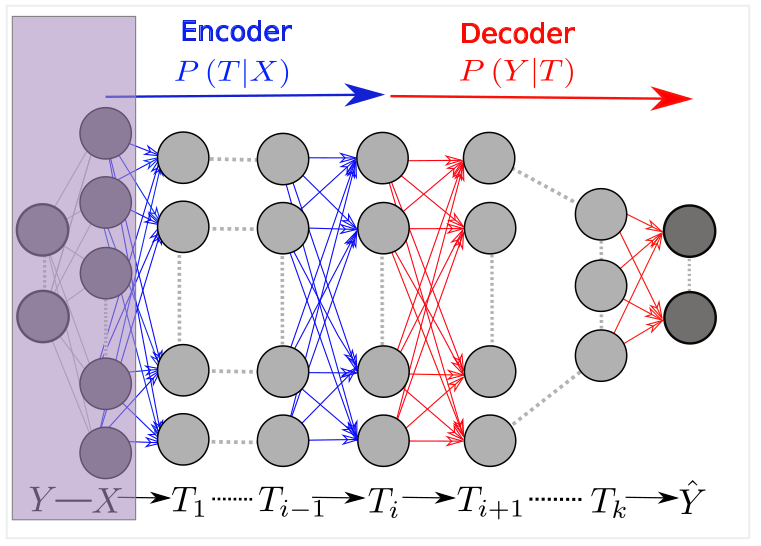
\includegraphics[width=0.8\textwidth]{MarkovChain.png}
	\end{figure}
\end{frame}

\begin{frame}
	\frametitle{Information Theory of Deep Learning 1}
	\footnotesize
	Mutual Information:
	\begin{equation}
		I(Input;Label) = D_{KL}[p(i,l)||p(i)p(l)] = \sum_{l \in Label; i \in Input} p(i,l) log\frac{p(i,l)}{p(i)p(l)}
	\end{equation}
	Invariance to invertible transformations: 
	\begin{equation}
		\forall \phi, \gamma: \exists \phi^{-1}, \gamma^{-1} \Rightarrow I(A;B) = I(\phi(A);\gamma(B))
	\end{equation}
	Data-Processing Inequality:
	\begin{equation}
		\forall X,Y,Z: (X \rightarrow Y \rightarrow Z) \Rightarrow I(X;Y) \geq I(X;Z)
	\end{equation}
\end{frame}

\begin{frame}
	\frametitle{Information Theory of Deep Learning 2}
	\footnotesize
	Minimal Sufficient Statistic:
	\begin{equation}
		T(Input) = \argmin_{S(Input):I(S(Input),Label)=I(Input, Label)} I(S(Input); Input)
	\end{equation}
	Information Bottleneck tradeoff:
	\begin{equation}
		\min_{p(r|i),p(l|r),p(r)} I(Input;Representation) - \beta I(Representation;Label)
	\end{equation}
	IB self-consistent equations:
	\begin{equation}
		\begin{cases}
			p(r|i) = \frac{p(r)}{Z(i;\beta)} exp(-\beta D_{KL}[p(l|i)||p(l|r)]) \\
			p(r) = \sum_{i}p(r|i)p(i) \\
			p(l|r) = \sum_{i}p(l|i)p(i|r)
		\end{cases}
	\end{equation}
	Optimal $\beta$ (relevance wheel):
	\begin{equation}
		\beta^{*}_j = \argmin_{\beta} \E D_{KL} [p_k(r|i) || p_{\beta}^{IB}(r|i)]
	\end{equation}
\end{frame}

\begin{frame}
	\frametitle{Network Behavior on Information Plane}
	\begin{figure}
		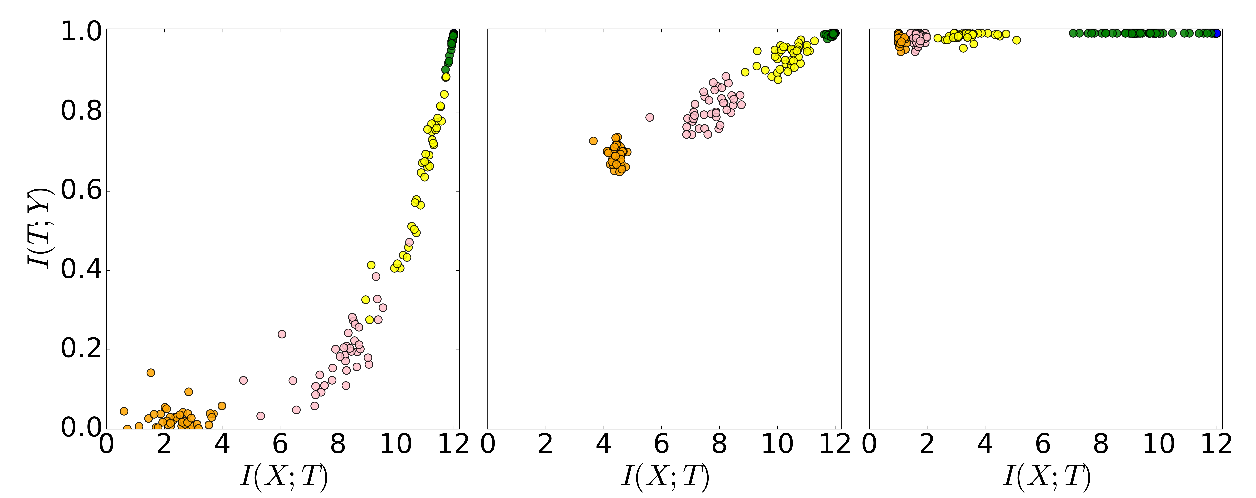
\includegraphics[width=\textwidth]{InformationPlane.png}
	\end{figure}
	\begin{itemize}
		\item First stage - compression of representation (from left to middle);
		\item Second stage - shuffling compressed representation to fit the labels (right);
	\end{itemize}
\end{frame}

\begin{frame}
	\frametitle{Consistency with theoretical boundaries}
	\begin{figure}
		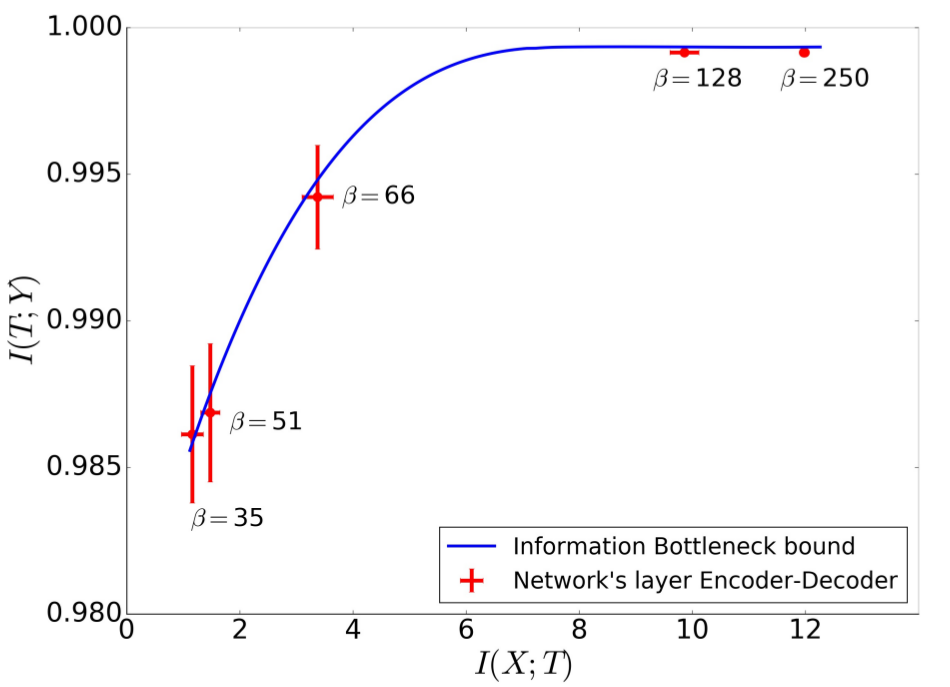
\includegraphics[width=0.8\textwidth]{TheoreticalBound.png}
	\end{figure}
\end{frame}

\begin{frame}
	\frametitle{Why do the networks need noise?}
	\begin{itemize}
		\item Mutual Information is invariant to any random shuffle of data;
		\item There is no way to distinguish between complex classes and simple classes (in terms of VC-dimension) by MI alone without tips on structure of those classes;
		\item The former is true only for deterministic functions;
		\item If the function is stochastic, the joint distributions can give a clue for distinguishing the classes.
	\end{itemize}
\end{frame}

\begin{frame}
	\frametitle{What's the point of hidden layers?}
	\tiny
	\begin{itemize}
		\item More hidden layers - good generalization is reached faster;
		\item Compression phase of a layer is shorter if it is started from previously compressed layer;
		\item For the deeper layers the compression is faster;
	\end{itemize}
	\begin{figure}
		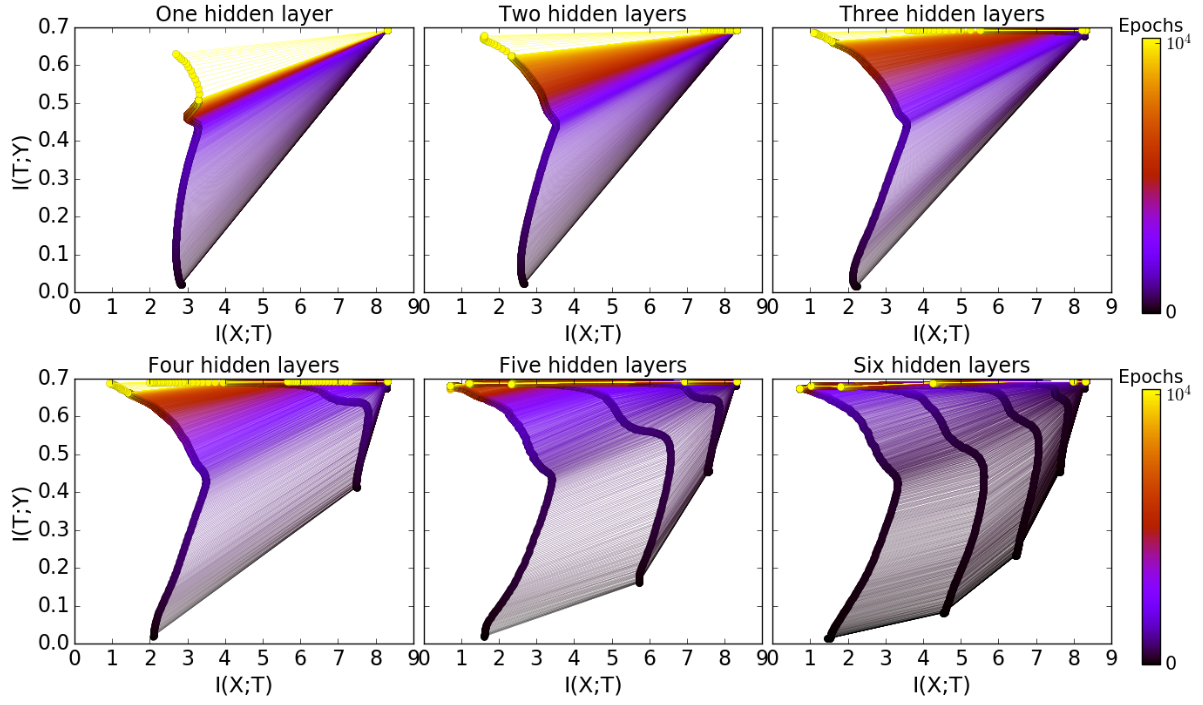
\includegraphics[width=\textwidth]{InformationPaths.png}
	\end{figure}
\end{frame}

\begin{frame}
	\frametitle{Numerical experiment setup}
	\begin{itemize}
		\item Different way of MI estimation - I use NPEET library;
		\item Real data instead of generated;
		\item Adam instead of plain SGD.
	\end{itemize}
	The models are trained on a subset of MNIST:
	\begin{itemize}
		\item 1000 - training sample size;
		\item 100 - test sample size.
	\end{itemize}
\end{frame}

\begin{frame}
	\frametitle{Numerical experiments on MNIST}
	\footnotesize
	The network used is fully-connected with 4 [256,128,64,32] hidden layers, trained to perform Regression (due to limitations of NPEET). Activations are ELU everywhere except the output layer which is Linear. The layer is marked by color in the following way: ["black", "red", "green", "blue", "yellow"].
	\begin{figure}
		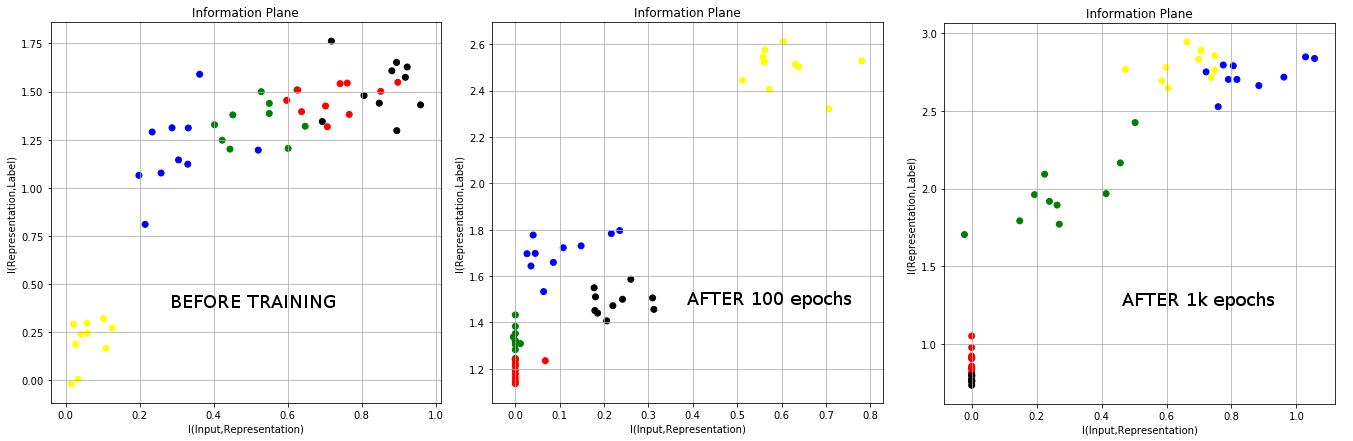
\includegraphics[width=\textwidth]{SnapshotReproduction.png}
	\end{figure}
	10 randomly initialized identical models are shown. The behavior is consistent with results of Schwarz-Ziv and Tishby. 
\end{frame}

\begin{frame}
	\frametitle{Interesting links}
	\begin{itemize}
		\item The paper of Schwarz-Ziv and Tishby - \url{https://arxiv.org/pdf/1703.00810.pdf};
		\item Non-Parametric Entropy Estimation Toolbox - \url{https://github.com/gregversteeg/NPEET};
		\item Deep Variational Information Bottleneck - \url{https://arxiv.org/pdf/physics/0004057.pdf};
		\item Code for numerical experiments in this presentation - \url{https://github.com/bakirillov/GM_Skoltech}.
	\end{itemize}
\end{frame}

\end{document}